\chapter{Simulating a Sociotechnical System for Healthcare}
\label{ch3}

\section{Introduction}
\label{ch3:intro}
This chapter concerns the simulation of a sociotechnical system in the domain of healthcare. In this case, we view a sociotechnical system as a large-scale information system, also called a societal information system, that gathers information from hundreds or thousands of individual entities with technical help. Such systems can be abstracted as graphs with nodes representing individual entities and edges representing relationships between them. The purpose of a sociotechnical system is to affect the behavior of a node by means of information retrieved from other nodes. Nowadays, a person's behavior is influenced by social networking services, such as Facebook. However, the amount of information to be comprehended and utilized in such services can be overwhelming for users. To further automate sharing and processing of information within a large social network or a sociotechnical system, we are investigating supporting each node in the network by a software agent. Software agents are autonomous computational entities that can be viewed as perceiving their environment through sensors and acting upon their environment through effectors. To say that agents are computational entities simply means that they physically exist in the form of programs that run on computing devices. To say that they are autonomous entities means that to some extent they have control over their behavior and can act without the intervention of humans or other systems. Agents pursue goals or carry out tasks in order to meet their design objectives, and in general these goals and tasks can be supplementary as well as conflicting \cite{huhns1999} \cite{wooldridge2009}. Agents can form commitments and act on behalf of individuals and form multiagent systems (MAS). We view agent-based sociotechnical systems as multiagent systems.

Sociotechnical systems are appropriate for a wide variety of problems, including regulation (e.g., banking), allocation of scarce resources (e.g., electric power and parking spaces), distributed situation assessment (e.g., urban air quality), system control (e.g., traffic management, both vehicular and telecommunication), and decentralized decision-making (e.g., choosing medical care). This article addresses simulating a sociotechnical system in the area of decentralized decision-making for healthcare.

Healthcare decision-making is done in many developed countries in the context of a healthcare quadruple, which consists of (1) patients, (2) healthcare providers (hospitals, health centers, labs, etc.) and provider networks, (3) insurance companies, and (4) the government. There is a variety of information systems available to support healthcare providers, provider networks, government healthcare agencies, and insurance companies, but none to support patients. Because patients are naturally distributed and are typically willing to assist each other, multiagent systems instead of centralized information systems would be appropriate for fostering this mutual assistance. In such systems, each patient would be represented by a software agent. The agent would assist its principal in health-related activities, such as understanding and interpreting insurance rules, finding the most cost-effective insurer, finding a good healthcare provider, providing advice on cost-effective drugs and care, and monitoring the spread of disease symptoms and their treatments. Feedback and information sharing among patients would be used extensively in such systems. Figure \ref{ch3:fmodelhealthcare} shows a sample situation of the proposed healthcare system. Patients shown on the right side of the figure are represented by agents, and each patient has friends with their acquaintanceship represented by edges. Patients may know some physicians, denoted by the edges between patients and physicians. Physicians has agents represent them too, and a physician may refer another physician.      

\begin{figure}
\centering
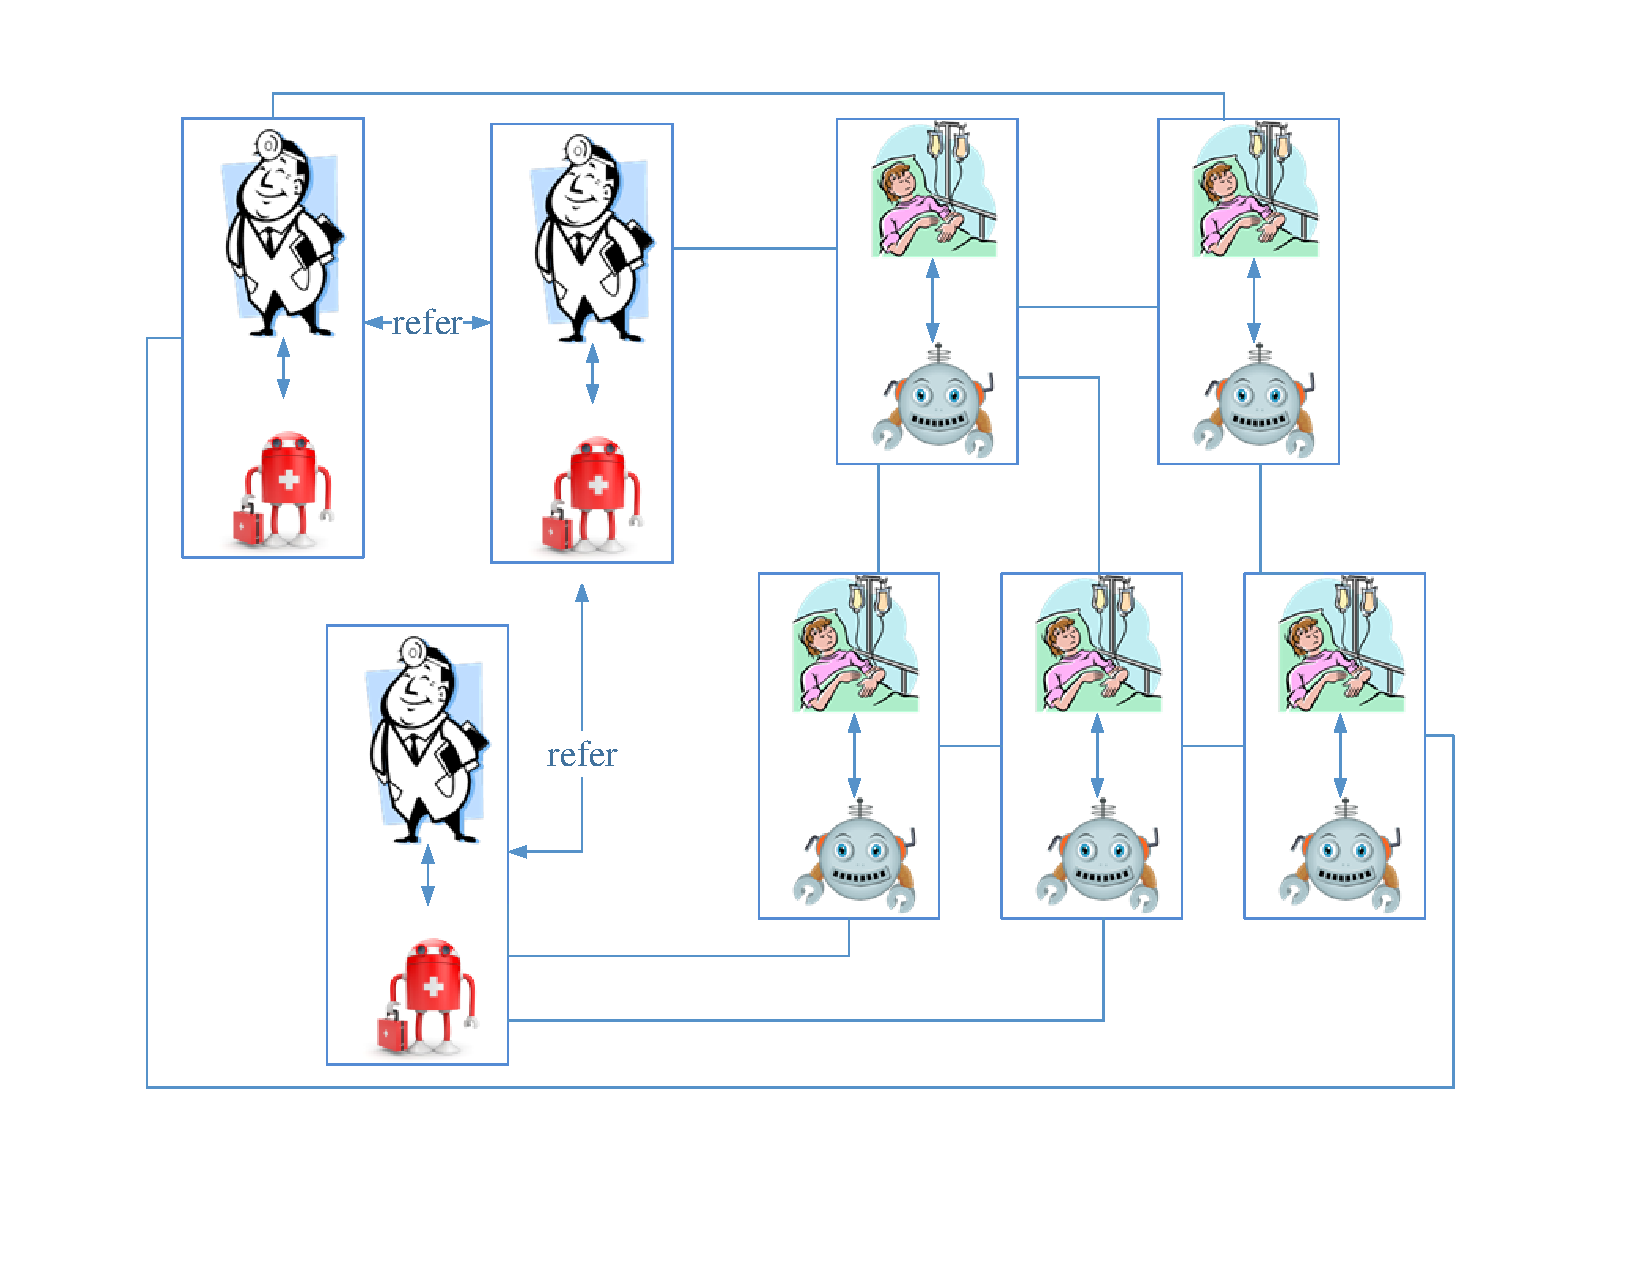
\includegraphics[scale=0.6]{chap3/chap3-model.pdf}
\caption{The model of the healthcare system}
\label{ch3:fmodelhealthcare}
\end{figure}

Investigating sociotechnical systems for healthcare is a broad research area. Moreover, it is difficult to experiment with such information systems in a society, especially because patients' health, privacy, and rights must be considered. We therefore have relied on simulations for prototyping and evaluating.

This chapter is organized as follows. First, we explain the method we use for prototyping the healthcare system - agent-oriented modeling. Second, we describe briefly how agent-oriented modeling is applied to design a simulated system for healthcare running on the NetLogo platform. Third, we analyze and explain the simulation results. We conclude by comparing the outcomes of using different choosing-a-physician strategies and waiting policies in the healthcare system and discussing the benefits of a sociotechnical system for healthcare.

\section{Related Work}
\label{ch3:relatedwork}
Multiagent systems are widely used in different areas, such as tracking goods, traffic control, consensus knowledge, and decision-making \cite{huhns2009}. One of the interesting areas for applying a MAS is healthcare.

Nealon and Moreno \cite{nealon2003} analyze features of healthcare problems, including the distributed nature of the knowledge that is needed to solve a problem, coordination, complexity, and so on. They claim that a MAS is an appropriate approach to tackle healthcare problems and could be used for patient scheduling, organ and tissue transplant management, community care, information access, and decision support systems. Isern et al. \cite{isern2010} compare the internal architecture and communication-based coordination techniques of fifteen healthcare-related agent-based systems and claim that agent-based systems increase reusability, flexibility, and other beneficial qualities as compared with centralized software systems, such as client-server systems.

MASs are also broadly used in home-care systems. Koutkias et al. \cite{koutkias2005} present a MAS for monitoring and detecting important cases for disease management. Isern et al. \cite{isern2008} describe the K4Care Home Care model, which uses an agent-based platform. Charfeddine \cite{charfeddine2010} introduces an agent-oriented framework to simulate the population of a chronic disease.

In the work most closely related to ours, Udupi and Singh \cite{udupi2010} use conceptual models in a sociotechnical system to implement a peer-to-peer network in which an agent contacts other agents to discover suitable service providers. It uses InterPol, a language and framework for supporting different kinds of interaction policies between agents. We described the modeling method of our sociotechnical system in \cite{taveter2012}.

There are several websites, similar to RateMDs \cite{ratemds}, where people rate doctors according to punctuality, medical knowledge, and other characteristics, and add comments. As we explain later, our approach differs from such websites and has advantages.

\section{Methodology}
\label{ch3:methodology}
We focuses on designing sociotechnical systems of a particular kind - sociotechnical systems for finding an appropriate physician and finding out the benefits to do so. We use the case study method \cite{taveter2012} and explore by rapid prototyping the design of a simulation of a sociotechnical system for healthcare. Rapid prototyping stands for implementing a proof-of-concept prototype in an agile way by directly mapping the modeling constructs to the constructs of a scripting environment like Netlogo or some agent-oriented environment like JADE. The method we use for prototyping is agent-oriented modeling. Agent-oriented modeling as described in \cite{sterling2009} is a holistic approach for analyzing, designing, and rapid prototyping of sociotechnical systems consisting of humans and technical components. We have chosen agent-oriented modeling because it is geared towards prototyping distributed systems that are open, adaptive, and intelligent. Sociotechnical systems are open systems because members of the society (e.g., commuters, patients, or shoppers) may join and leave the system at any time. Sociotechnical systems are adaptive systems, because they should react to their constantly changing environment, which for example can take the form of changes in traffic infrastructure, health insurance coverage, and product prices. We also term sociotechnical systems as intelligent systems, because they reflect the "wisdom of crowds" when recommending a patient, for example, a healthcare provider. In addition, agent-oriented modeling meets well the requirements for purposefulness and understandability of the design.

A set of canonical models are introduced in agent-oriented modeling, whose types are shown in Table \ref{ch3:tmodeltypes}. In addition to representing each model with an abstraction layer (analysis, design, or prototyping), Table \ref{ch3:tmodeltypes} maps each model to the vertical viewpoint aspect of interaction, information, or behavior. Each cell in the table represents a specific viewpoint. We explain these viewpoints in the following paragraphs.

\begin{table}[!t]
\caption{The model types of agent-oriented modeling}

\centering
\begin{tabular}{|c|c|c|c|} 
\hline

& \multicolumn{3}{c|}{\textbf{Viewpoint aspect}}\\ \hline
\textbf{Abstraction layer} & Interaction & Information & Behavior\\ \hline
\multirow{2}{*}{Analysis} & Role models and & \multirow{2}{*}{Domain model}& \multirow{2}{*}{Goal models}\\  
 &organization model & & \\
\hline
\multirow{2}{*}{Design} & Agent models and & Knowledge& Behavioral \\
 & interaction models&  models& scenarios\\ 
\hline
\multirow{2}{*}{Prototyping} & Interaction & Information & Behavior \\ 
 & prototyping & prototyping& prototyping\\ 
\hline
\end{tabular}
\label{ch3:tmodeltypes}
\end{table}

From the viewpoint of interaction analysis, role models represent the properties of roles and the relationships between the roles are represented by an organization model. From the viewpoint of information analysis, a domain model represents the knowledge to be handled by the sociotechnical system. From the viewpoint of behavior analysis, a goal model is a container of three components: goals, quality goals, and roles.  

From the viewpoint of interaction design, agent models transform the abstract constructs from the analysis stage, roles, to design constructs, agent types, which will be realized in the implementation process. Interaction models are used to express interaction patterns between agents. From the viewpoint of information design, knowledge models represent both private and shared knowledge of agents. From the viewpoint of behavior design, behavioral scenarios are used to show how agents make decisions and perform activities \cite{taveter2012j}.

Modeling at the abstraction layer of prototyping is explained in section \ref{ch3:evaluation}.

Figure \ref{ch3:fgoalmodel} shows the goal model of our sociotechnical system for healthcare, in which rectangles stand for functional goals and clouds stand for quality goals. The stick figures represent roles that are required for achieving the goals. As can be seen from Figure \ref{ch3:fgoalmodel}, from the viewpoint of behavior analysis, our sociotechnical healthcare system focuses on the purpose of "Allocate Healthcare Resources" among the members of the society. Specifically, we study the allocation of physicians - a special kind of healthcare resource. Achieving the functional goal "Allocate Healthcare Resources" is characterized by the quality goal "Maximal Societal Health", which determines the quality criterion according to which healthcare resources should be allocated in a society.

\begin{figure}
\centering
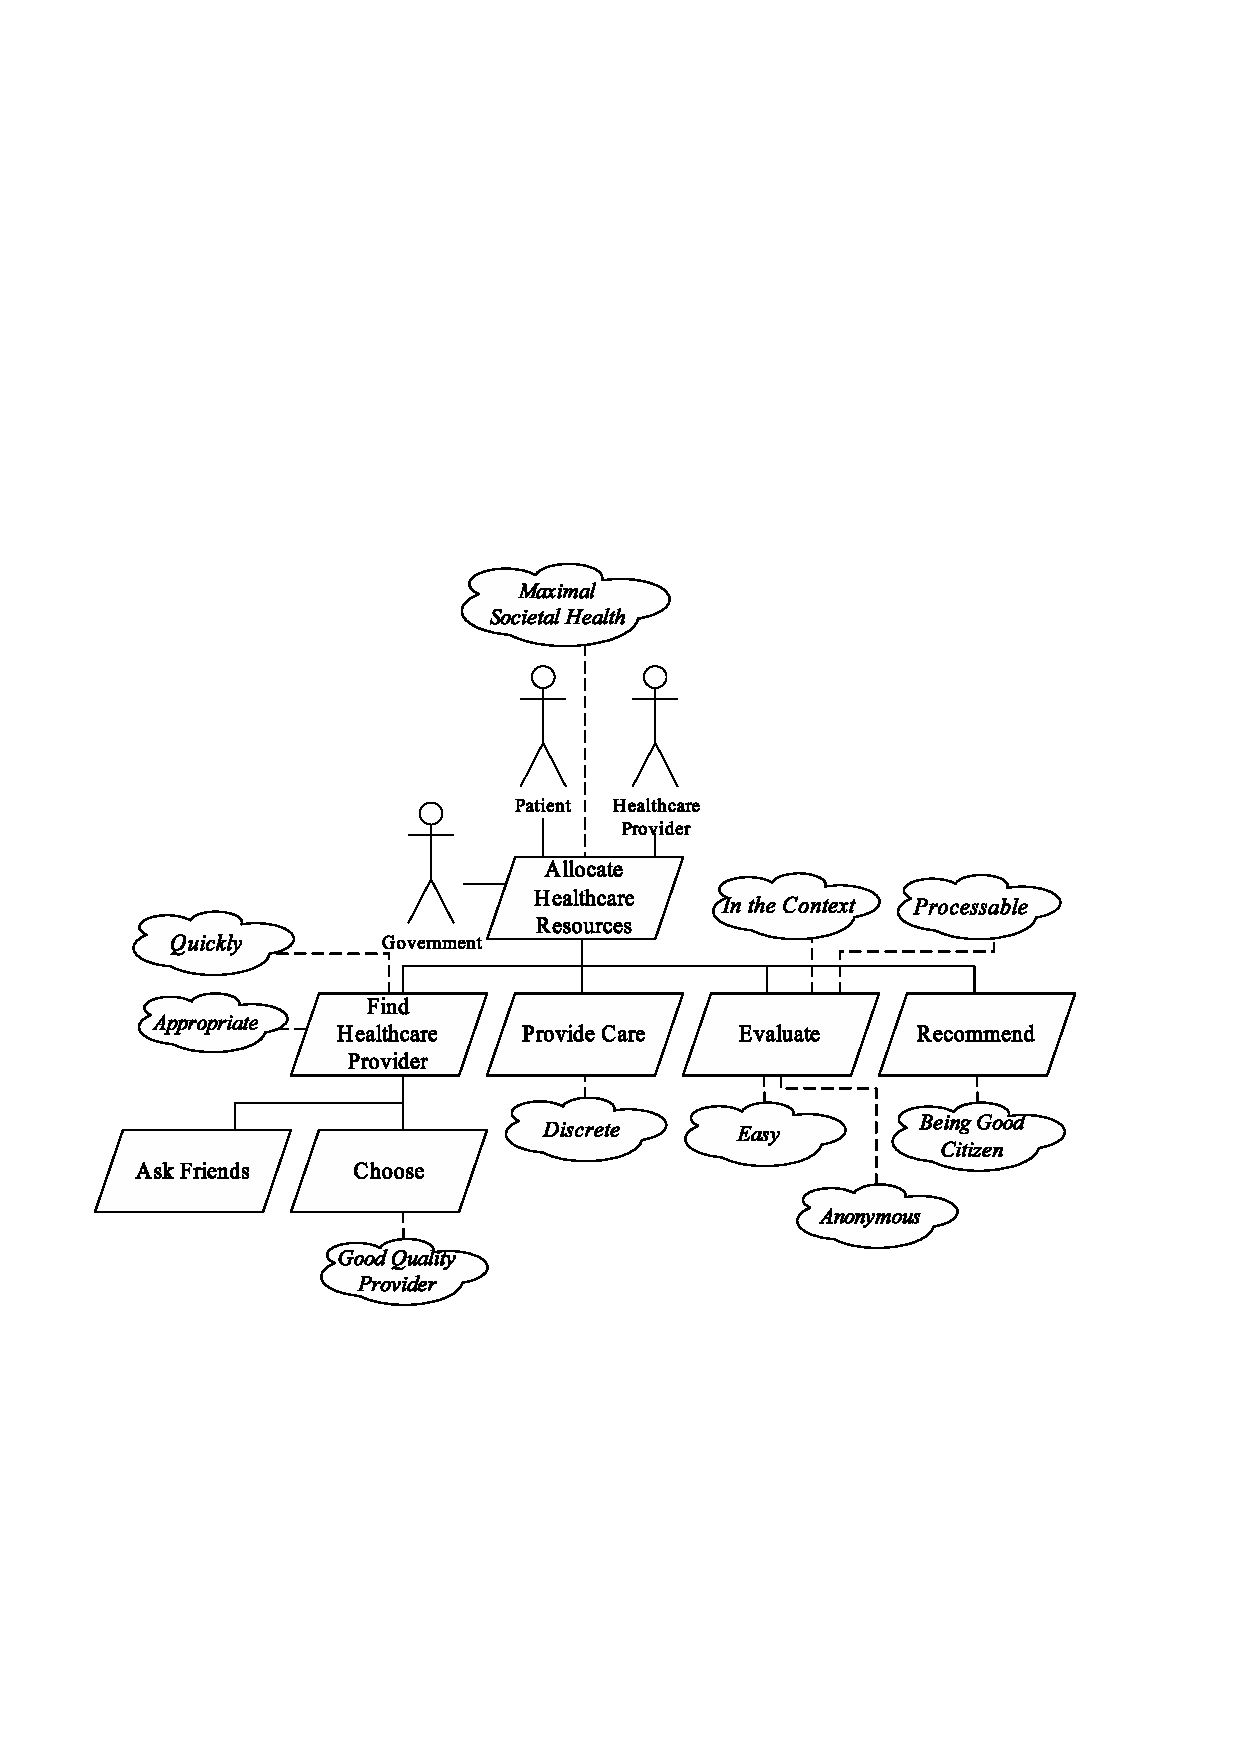
\includegraphics[scale=0.7]{chap3/chap3-fgoalmodel.pdf}
\caption{The goal model of the healthcare system}
\label{ch3:fgoalmodel}
\end{figure}

To accomplish the purpose "Allocate Healthcare Resources" of the sociotechnical system, its four subgoals need to be achieved: finding a healthcare provider, being provided with care, evaluating the care, and recommending healthcare providers to other patients. As we demonstrate below, to fulfill the goal "Find Healthcare Provider", a patient recursively asks her friends, friends' friends, and so forth for recommendations and chooses the best physician recommended. This is represented as two subgoals of "Find Healthcare Provider:" "Ask Friends" and "Choose."

We attach a number of quality goals to the functional goals in the goal model. The meanings of the quality goals are easy to understand. For example, "Quickly" means a patient wants to find a healthcare provider as soon as possible. The "Anonymous" quality goal expresses that no evaluation by a patient should identify the patient. It should be noted that the quality goal "In the Context" attached to the functional goal "Evaluate" represents that evaluation has to occur in the context of receiving the service, preferably before leaving the facilities of the healthcare provider or at least on the same day. The "Processable" quality goal means that the evaluation should be presented in a form amenable to computer processing. In our simulation, we use a scale from 1 to 5 to measure the evaluations.

According to Figure \ref{ch3:fgoalmodel}, we model two roles for our simulation - Patient and Healthcare Provider. There is also a third role - Government. Since our work focuses on the particular aspect of the U.S. healthcare domain dealing with how a patient finds a physician, rather than modeling the healthcare domain in its full complexity, the Government role's modeling is not relevant to the simulation system being designed and we ignore the Government role in our system. Additionally, we complement the goal model with the new Assistant role, which is not shown in Figure \ref{ch3:fgoalmodel}. The Assistant role is the assistant of a person and is responsible for asking friends for recommendations, choosing a healthcare provider, and assisting in evaluating the care. In the prototypical system being designed, the role of Assistant should obviously be mapped to the Assistant Agent software agent type. Since a patient is a real human that is treated by another real human - a physician - we map both the roles Patient and Healthcare Provider to the Human Agent type. The software system boundary of the sociotechnical system is obviously between the roles Patient and Assistant.

From the viewpoint of interaction analysis, the organization model of the sociotechnical system being designed is decided based on the three kinds of networks that are used for representing the relationships among the members of the society as follows. Also, we make the average degree of the three networks equal to or almost equal to a certain number, which is 6 in our case, in order to reduce the difference among different network models. The average degree of a graph is defined as $2*|E|/|V|$, where $|E|$ is the number of edges and the $|V|$ is the number of vertices in the graph.
\begin{itemize}
\item[-]Random network: the relationships between pairs of patients are created randomly until the desired number, which is 3 times of the number of nodes, to ensure the average degree is 6.
\item[-]Small-world network: most nodes are not neighbors to one another, but most nodes can be reached from any other node by a small number of hops. We followed the approach in \cite{watts1998} to construct our network by first organizing the vertices into a circle, connecting each vertex to its 3 nearest neighbors and then rewiring each edge between the vertex in question and its $k$th nearest neighbor with a 20\% probability, where $k=1, 2, 3$ for all the vertices in the graph. Edges which satisfy the condition that $k$ equals to a certain number should be rewired first and then the procedure goes on with next available $k$. The average degree is 6 in the small-world network.
\item[-]Scale-free network: the shortest paths between nodes flow through hubs, and if a peripheral node is deleted, it is unlikely that this will interfere with passing a message between other peripheral nodes. We use the Barab{\'a}si-Albert model \cite{barabasi1999} to construct a scale-free network for our simulation. Starting with two nodes, we keep adding a new node and 3 edges which connect the new node with three nodes that are already in the graph each time until we reach the desired number of nodes. For the edges, the probability of connecting with a certain node $i$ in the graph depends on the connectivity or degree of the node $k_i$ such that the probability is $k_i/\sum_{j}k_j$. For the first new node added, we add two edges because there are only two nodes in the graph in the beginning. The average degree of the scale-free network is 5.998, which is very close to 6. A scale-free network is a common model for a collaboration network.
\end{itemize}
We have shown examples of the three different networks in Figure \ref{ch3:fnetworks}. The number of persons is 15 and the average degree is 4 in these networks. The edge between two persons means they know each other.

\begin{figure}
\centering
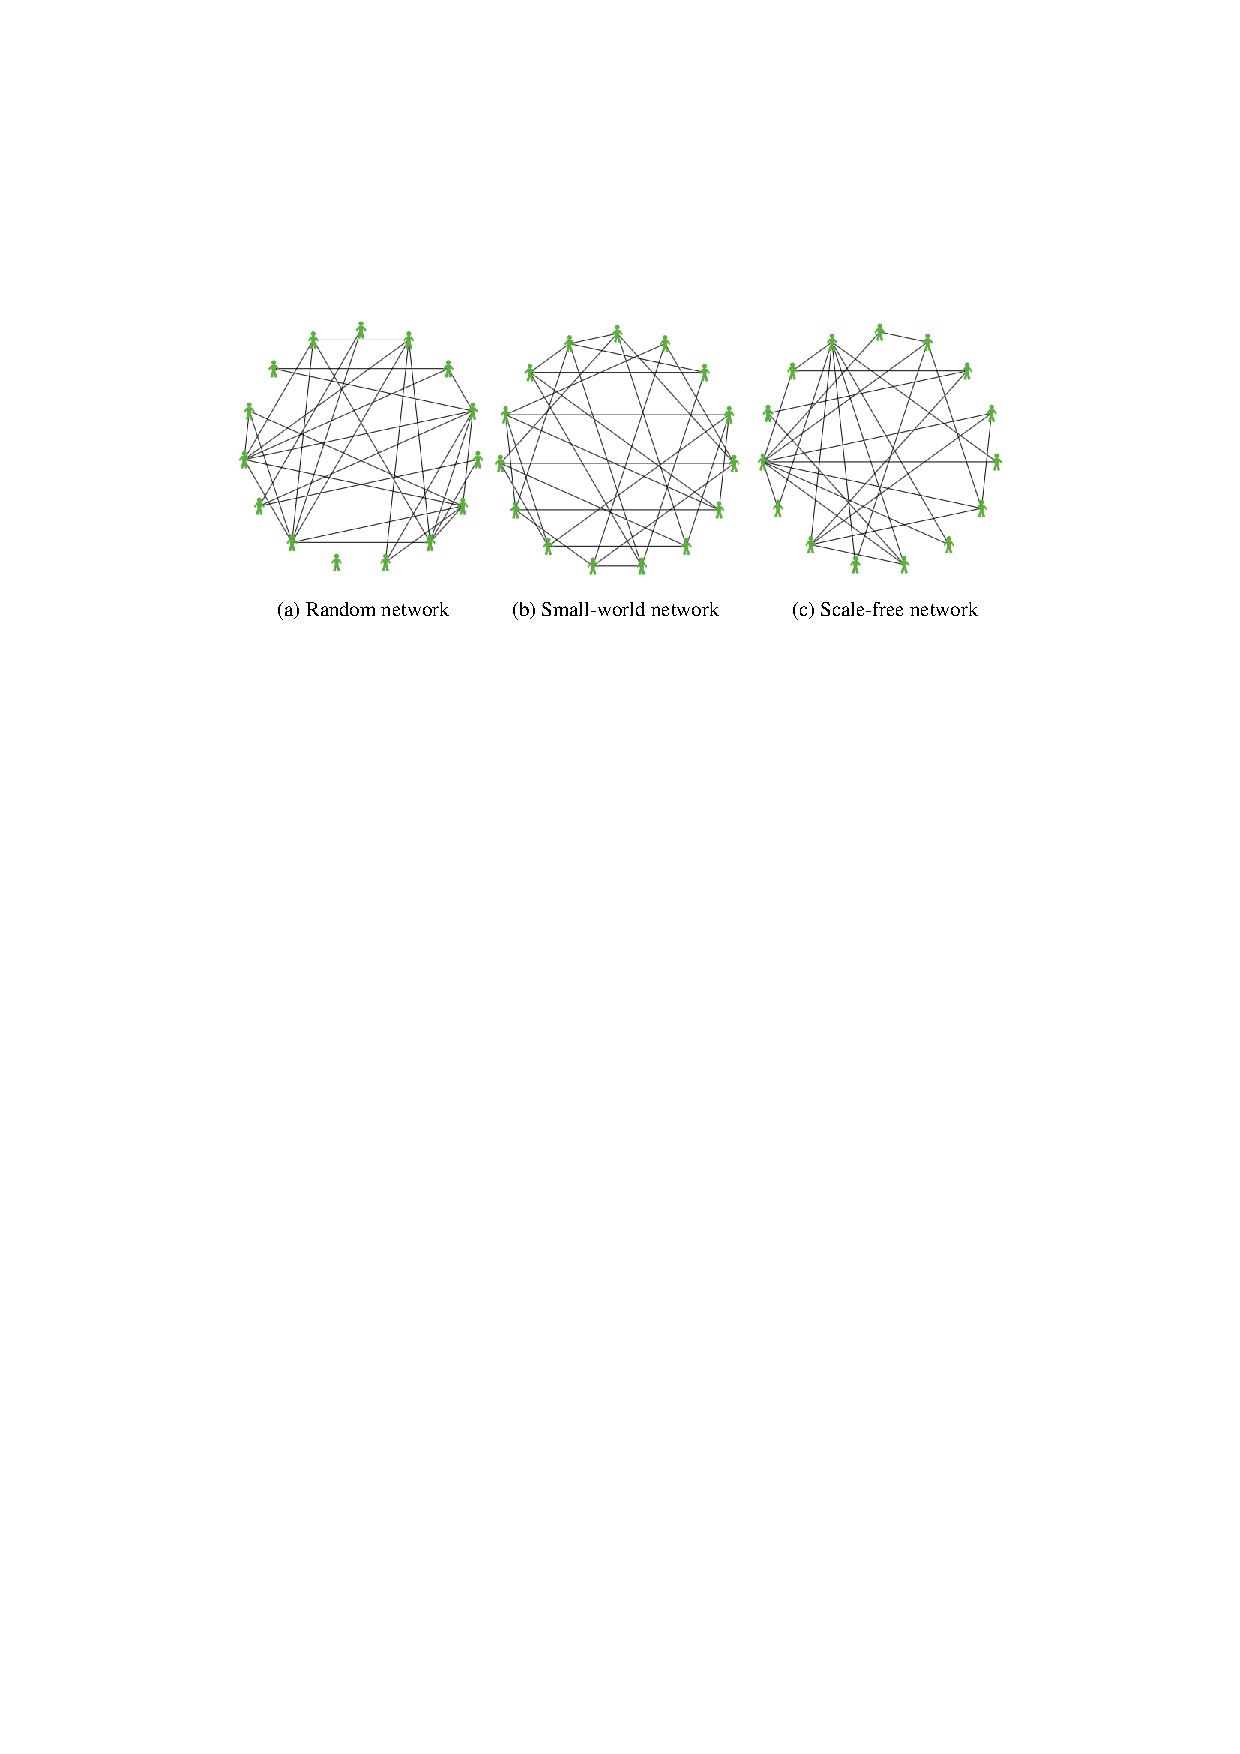
\includegraphics[scale=1]{chap3/chap3-fnetworks.pdf}
\caption{Different networks}
\label{ch3:fnetworks}
\end{figure} 
	
After covering the viewpoints of behavior analysis and interaction analysis, we next proceed to the viewpoint of information analysis by addressing the knowledge to be represented within the system. We do this by identifying the types of knowledge entities related to the roles. As each healthcare provider has predefined capacity and efficiency, which are explained in section \ref{ch3:evaluation}, we attach the Capacity and Efficiency knowledge entity types to the Healthcare Provider role.

We now proceed to the viewpoint of interaction design. Finding a physician involves interactions between Assistant Agents representing patients. We represent these interactions as an interaction protocol between agents of the type Assistant Agent. It is appropriate to remind here that the difference between an interaction protocol and other kinds of interaction models is that an interaction protocol models some aspects of the agent behaviors along with their interactions \cite{sterling2009}.

Representing the interaction protocol of the sociotechnical system is very important, because it describes the patient's strategy of choosing a physician. We explored the following four possible choosing-a-physician strategies:
\begin{itemize}
\item[-]Random strategy. The patient's Assistant Agent randomly chooses a physician.
\item[-]The "Choose one" strategy. The patient's Assistant Agent chooses the best physician according to the patient's evaluations and his friends' evaluations. Besides the physician(s) with the best evaluation the patient already knows, his Assistant Agent asks his friends' Assistant Agents for recommendations. An Assistant Agent acting on behalf of the patient's friend may deal with the request in one of the following ways:

\begin{itemize}
\item[-]Reply with the physician(s) who has the best evaluation.
\item[-]Provide the requesting agent with the address of the Assistant Agent of one of its principal's friends if there is no recommendation to give. This process continues recursively until the first recommendation is received or until all the friends down to the maximum forwarding depth have been asked. The forwarding depth is defined as follows: the originator's friends are at depth 1; the originator's friends' friends at depth 2, and so on.
\end{itemize}

Figure \ref{ch3:fprotocol} presents the interaction protocol among patients' Assistant Agents for the "Choose one" strategy. It models that the Assistant Agent of a patient's friend may respond with a recommendation or recommend the Assistant Agent of the friend's friend. This means the interaction protocol is recursive, which is represented by the "Loop" behavioral construct. A friend's Assistant Agent may also ignore a request, which is not shown in the figure.
\end{itemize}

\begin{figure}
\centering
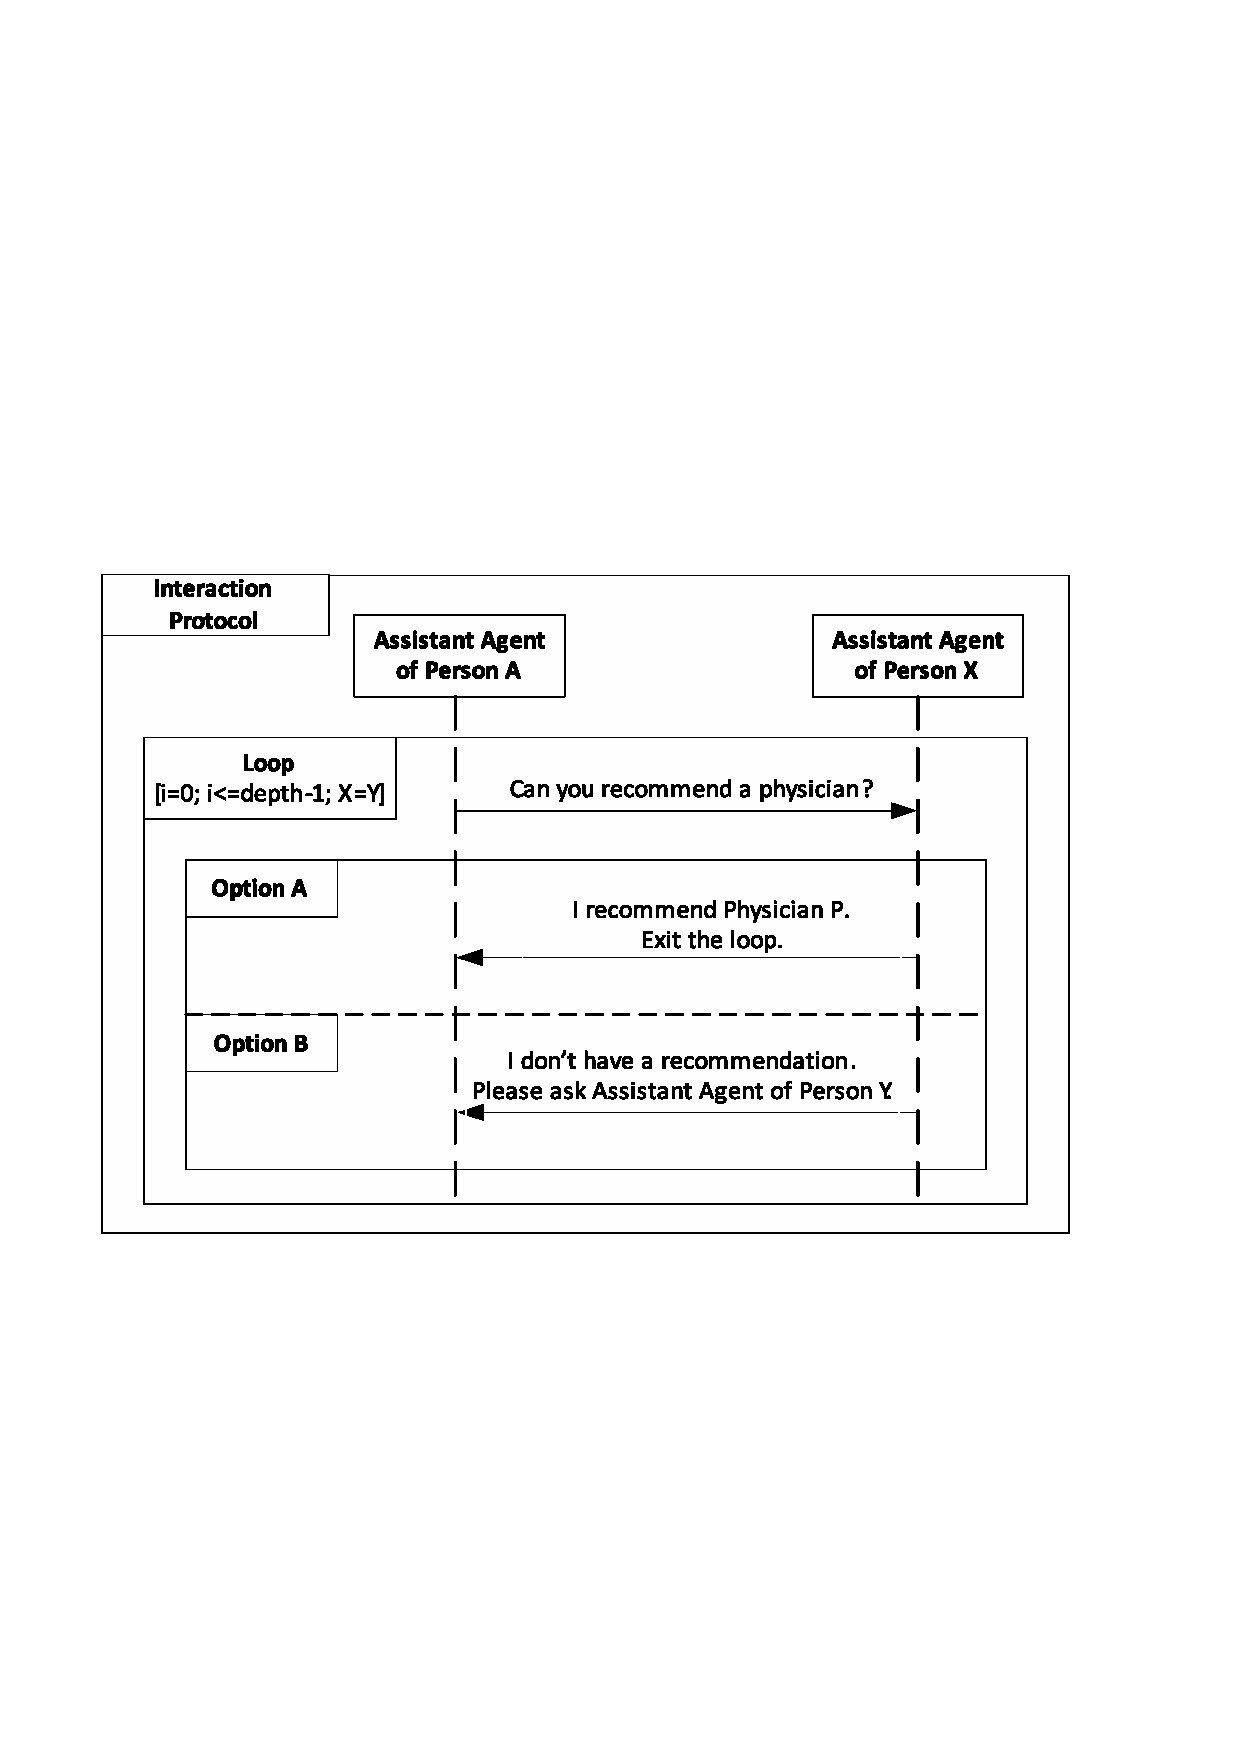
\includegraphics[scale=0.7]{chap3/chap3-fprotocol.pdf}
\caption{The interaction protocol for "Choose one" strategy}
\label{ch3:fprotocol}
\end{figure}

In addition to the random and "Choose one" strategies, we have included in our simulations the "Borda voting" and "Add and minimize" strategies. These strategies are briefly described as follows:
\begin{itemize}
\item[-]The "Borda voting" strategy. The patient's Assistant Agent asks his friends' Assistant Agents, who are closer than a specified limit in depth, for recommendations. A friend's Assistant Agent may choose to not answer, or tell the patient's Assistant Agent what it knows about all the physicians. After the patient's Assistant Agent has received all the responses, it calculates for each physician the Borda count [a single-winner election method in which voters rank candidates in order of preference, named for the 18th-century French mathematician and political scientist Jean-Charles de Borda, who devised the system in 1770], according to which a physician is given a number of points equal to the number of physicians whose evaluations are worse than the evaluations of the given physician. Thereafter the agent adds up all the points gained by the physician in question. The physician with the highest score is chosen.
\item[-]The "Add and minimize" strategy, which has the same procedure for getting recommendations as the "Borda voting" strategy. After the patient's Assistant Agent has received all the responses, it adds up all the nonzero evaluations and calculates the mean value of them for each physician. Then the Assistant Agent chooses the physician with the minimum mean evaluation. Choosing the physician with the minimum value is due to the way we define the evaluation, as described in section \ref{ch3:evaluation}.
\end{itemize}

To make it clear, Figure \ref{ch3:fchoosephysicianeg} shows an example. In the figure, a red-border box means the agent with its principle ignores the request when asked for recommendation (Allan and Erle); green means it wants to reply and it has some information (Bob, Conan, Flora and Gabby); purple means it wants to reply but it has no information (Daniel and Harris). In the "Choose one" strategy, Paul's agent asks agents of all his friends, Allan, Bob, Conan, and Daniel. Allan's agent doesn't reply for this time. Agents of Bob and Conan reply with the evaluations of the best physician(s) they know. Daniel's agent wants to reply, but it doesn't have any information. Thus, it gives Paul's agent the addresses of the agents of Daniel's friends, Gabby and Harris. Paul's agent asks Gabby's agent for recommendation and Gabby's agent replies with the best physician it knows, then Paul's agent won't ask Harris's agent any more. In the "Borda voting" and "Add and minimize" strategy, Paul's agent will ask agents of all the other persons in the figure if the depth limit is set to 2, gather evaluations of all the physicians from them and integrate these information to make a suggestion. 

\begin{figure}
\centering
\includegraphics[scale=0.7]{chap3/chap3-choosephysicianEg.pdf}
\caption{An example of different strategies}
\label{ch3:fchoosephysicianeg}
\end{figure}	
   	
From the viewpoint of behavior design, to model the behaviors of agents of the decided types, we transform responsibilities of the roles into activities attached to the agent types. As a result, we obtain behavioral scenarios for agents playing the roles Patient, Assistant, and Physician. For example, the behavioral scenario of an agent of the type Assistant Agent playing the role Assistant models that the activities "Find a physician" and "Evaluate" are performed sequentially. In a sociotechnical system for healthcare this is always the case, because the Assistant Agent does not perform any activities between these activities while a patient is attended by a physician.

Another aspect of the Assistant Agent's behavior in choosing a physician deals with what the agent should do if the physician is not available on the given day. We have decided to consider the following three waiting policies, which, for instance, could be decided by the patient's insurance company:
\begin{itemize}
\item[-]Waiting. The patient's Assistant Agent chooses the best physician by adopting one of the choosing-a-physician strategy explained above and sticks to this choice. If the physician is busy, the patient will still make an appointment with the physician and will wait until the physician becomes available.
\item[-]No waiting. If the physician chosen is busy, the patient's Assistant Agent will choose a physician randomly according to the "Random" strategy or the next best physician according to the other choosing-a-physician strategies until it finds an available physician.
\item[-]Waiting with limit. If the physician chosen is not available, the patient's Assistant Agent will check whether the physician could be reached in a certain number of days. If it is possible, the patient will make an appointment and wait. If not, the Assistant Agent will choose another physician according to the rules of the same waiting policy. If no physician is available in a certain number of days, the Assistant Agent will choose a physician who has the smallest number of days required for waiting.
\end{itemize}	
	
Finally, distinguishing between private and public knowledge entities from the viewpoint of information design is straightforward, because the knowledge entity Evaluation is private to the patient and Assistant Agent helping him/her, while the knowledge entity Recommendation is shared between different patients and instances of Assistant Agent. Similarly, the knowledge entity Efficiency is private to each Healthcare Provider, but at the same time naturally forms a basis for how patients evaluate healthcare providers. We describe models including role models, the organization model, and the domain model in detail in \cite{taveter2012}.

\section{Evaluation}
\label{ch3:evaluation}
\subsection{Simulation Settings}
We next describe from the three viewpoints introduced in section \ref{ch3:methodology} how we mapped agent-oriented models of the sociotechnical system to the programming constructs of the simulation environment.

From the viewpoint of information prototyping, we represented the knowledge entities decided by agent-oriented modeling as described in section \ref{ch3:methodology} as follows:
\begin{itemize}
\item[-]The Capacity knowledge entity - in terms of the number of patients per day that a given physician can handle.
\item[-]The Efficiency knowledge entity - in terms of the number of days that it takes for a given physician to cure a patient. This number of days is generated for each physician according to a normal distribution whose mean and standard deviation can be adjusted in the user interface.
\item[-]The Evaluation knowledge entity - in terms of the following variables:
\begin{itemize}
\item[-]The number of days the physician in question failed to handle a given patient. How this value is determined is explained below.
\item[-]The number of days that the physician needed to cure a patient. This is determined by the Efficiency knowledge item pertaining to the physician.
\item[-]A random component representing that different patients evaluate the same physician differently.
\end{itemize}
\end{itemize}
	
A patient's evaluation for a specific physician is calculated by adding these three factors. For example, let us assume that a patient gets sick today and decides to visit a physician chosen by her Assistant Agent, but the physician is busy and cannot see the patient until tomorrow. In this case, the value of the first factor - the number of days the physician in question failed to handle a given patient - is 1, because the patient had to wait for 1 day to see the physician. The second factor - the number of days that the physician requires to cure the patient - is a fixed number related to the physician in question. The third factor - the random component expressing the subjective factor - is a random value that varies between -0.5 and 0.5.

The viewpoint of behavior prototyping covers the behaviors of software agents representing patients and physicians. In accordance with the behavioral scenarios modeled as a part of the design described in section \ref{ch3:methodology}, every day the patients each try to decide which physician to visit. For each patient, the Assistant Agent acting on behalf of its principal may ask Assistant Agents of the principal's friends for recommendations and then makes a decision as to which physician the principal should visit.

From the viewpoint of interaction prototyping, the exchange of messages to be implemented is modeled according to interaction diagrams, such as the one in Figure \ref{ch3:fprotocol} for the case of choosing a physician according to the "Choose one" strategy. To make our simulations more realistic, we have chosen a 20\% probability that a friend would ignore the patient's request.

Back to the viewpoint of behavior prototyping, the software agent corresponding to the Assistant Agent recommends physicians based on evaluations. The agent can recommend only those physicians that its principal has actually visited in the simulation. The number of days the physician in question could not handle the given patient, because of the physician's exceeded capacity, accumulates in the patient's evaluation until the patient actually visits the given physician. On each new visit the agent "forgets" its previous evaluation and updates its knowledge base with the new evaluation. The reason why the agent forgets its previous evaluation is that during the time period between the previous evaluation and the new evaluation, factors that influence the evaluation may have occurred. For example, the physician may have become more skilled. Therefore it is fairer to use the latest evaluation.

To make our simulations as realistic as possible, we used the following statistical data by the Centers for Disease Control and Prevention (CDC) from the year 2008 \cite{visit}:
\begin{itemize}
\item[-]The number of physician office visits per 100 people per year: 320.1.
\item[-]The number of physicians per 10,000 people: 26.
\end{itemize}
	
Based on the above data, we obtained the average number of people who get sick every day by dividing the number of visits per 10,000 people by 250, which is the standard number of working days in a calendar year in the U.S. As a result, 128 people out of a population of 10,000 get sick every day.

\subsection{Results and Evaluation}
We simulated 365 days with 5,000 patients and 13 physicians. In our simulation, 64 random people get sick every day. The value of the local variable of each physician's software agent corresponding to the Capacity knowledge entity was set to 8 patients per day. The value of the local variable of each physician's software agent corresponding to the Efficiency knowledge entity was determined randomly according to a normal distribution with mean value 3 days and with the value of deviation as 2.0.

Figure \ref{ch3:fdays} describes the number of days needed for curing by different physicians in our simulations.

We performed simulations by combining the types of social networks with different choosing-a-physician strategies and waiting policies, which are described in section \ref{ch3:methodology}. The results from simulations in terms of the annual sick days per person and leftover patients who were not taken care of by the end of the last day simulated are represented in Tables \ref{ch3:tdran} - \ref{ch3:tpscale}.

\begin{figure}
\centering
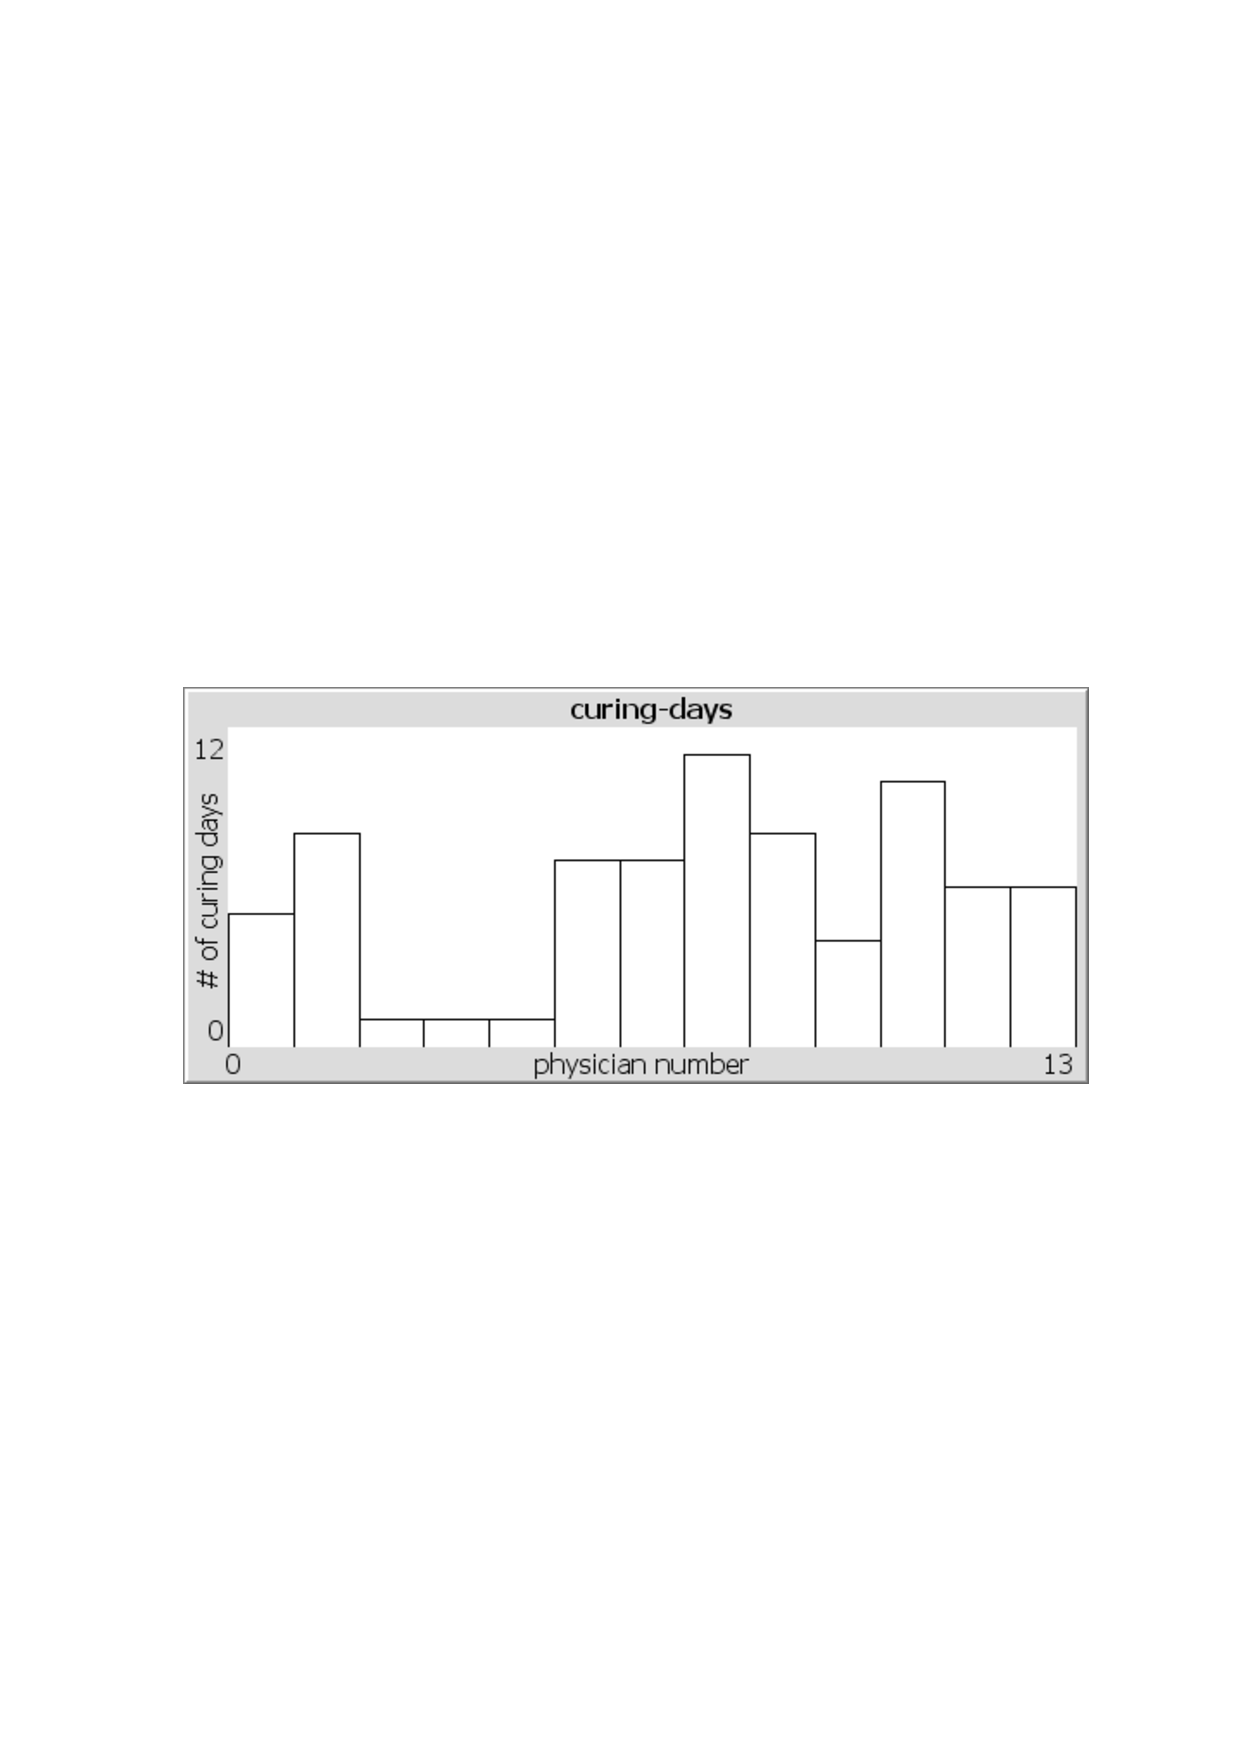
\includegraphics[scale=0.6]{chap3/chap3-fdays.pdf}
\caption{Days needed to be cured by different physicians}
\label{ch3:fdays}
\end{figure}

\begin{table}[!t]
\centering
\caption{Average sick days for random network}

\begin{tabular}{|c|c|c|c|}
\hline
& \multicolumn{3}{c|}{\textbf{Waiting policy}}\\ \hline
\textbf{Choosing-a-physician strategy}
& Waiting & No waiting & Waiting with limit\\ \hline
Random&  6.8&  6.8& 6.8\\ \hline
Choose one& 12.2 &  5.2& 6.3\\ \hline
Borda voting& 34.8 & 6.0 & 8.3\\ \hline
Add and minimize & 10.2 & 4.9 & 6.4\\ \hline
\end{tabular}
\label{ch3:tdran}
\end{table}

\begin{table}[!t]
\centering
\caption{Leftover patients for random network}

\begin{tabular}{|c|c|c|c|}
\hline
& \multicolumn{3}{c|}{\textbf{Waiting policy}}\\ \hline
\textbf{Choosing-a-physician strategy}
& Waiting & No waiting & Waiting with limit\\ \hline
Random&  0&  0& 0\\ \hline
Choose one&  427&  0& 80\\ \hline
Borda voting&  4569&  0& 96\\ \hline
Add and minimize & 155 &  0& 94 \\ \hline
\end{tabular}
\label{ch3:tpran}
\end{table}


\begin{table}[!t]
\centering
\caption{Average sick days for small-world network}

\begin{tabular}{|c|c|c|c|}
\hline
& \multicolumn{3}{c|}{\textbf{Waiting policy}}\\ \hline
\textbf{Choosing-a-physician strategy}
& Waiting & No waiting & Waiting with limit\\ \hline
Random&  6.8&  6.8& 6.8\\ \hline
Choose one& 10.3 & 5.2 & 6.3\\ \hline
Borda voting& 7.6 & 6.6 & 6.8\\ \hline
Add and minimize & 9.6 & 5.0 & 6.3\\ \hline
\end{tabular}
\label{ch3:tdsmall}
\end{table}

\begin{table}[!t]
\centering
\caption{Leftover patients for small-world network}

\begin{tabular}{|c|c|c|c|}
\hline
& \multicolumn{3}{c|}{\textbf{Waiting policy}}\\ \hline
\textbf{Choosing-a-physician strategy}
& Waiting & No waiting & Waiting with limit\\ \hline
Random& 0 & 0 & 0\\ \hline
Choose one& 407 & 0 & 71\\ \hline
Borda voting& 76 & 0 & 25\\ \hline
Add and minimize & 239 & 0 & 93\\ \hline
\end{tabular}
\label{ch3:tpsmall}
\end{table}


\begin{table}[!t]
\centering
\caption{Average sick days for scale-free network}

\begin{tabular}{|c|c|c|c|}
\hline
& \multicolumn{3}{c|}{\textbf{Waiting policy}}\\ \hline
\textbf{Choosing-a-physician strategy}
& Waiting & No waiting & Waiting with limit\\ \hline
Random& 6.8 & 6.7 &6.8 \\ \hline
Choose one& 13.7 & 5.3 & 6.3\\ \hline
Borda voting& 38.6 & 6.5 & 9.9\\ \hline
Add and minimize & 9.4 & 4.9 & 6.4 \\ \hline
\end{tabular}
\label{ch3:tdcale}
\end{table}

\begin{table}[!t]
\centering
\caption{Leftover patients for scale-free network}

\begin{tabular}{|c|c|c|c|}
\hline
& \multicolumn{3}{c|}{\textbf{Waiting policy}}\\ \hline
\textbf{Choosing-a-physician strategy}
& Waiting & No waiting & Waiting with limit\\ \hline
Random& 1 & 0 & 2\\ \hline
Choose one& 686 & 0 & 78\\ \hline
Borda voting& 4449 & 0 & 110\\ \hline
Add and minimize & 255 & 0 & 96\\ \hline
\end{tabular}
\label{ch3:tpscale}
\end{table}

We can see from Tables \ref{ch3:tdran} - \ref{ch3:tpscale} that if a patient follows the "Waiting" policy, the "Random" strategy will outperform all the other choosing-a-physician strategies in social networks of all three kinds addressed. This is the case because in all the other strategies, a patient always waits for the best physician chosen by her Assistant Agent, which increases the waiting days and accordingly sick days. Also, because the Random strategy leads to even visiting of physicians, it has no leftover patients, but there are leftover patients in the other three strategies.  

The performance of the "Borda voting" strategy is the worst in all three kinds of social networks addressed, except for the combination of the "Borda voting" strategy and "Waiting" policy in the small-world network, because it uses more evaluation information than the other strategies due to its method for calculating the votes for physicians. 

Differently from the "Borda voting" strategy, the "Add and minimize" strategy uses less information because it does not consider the physicians who have not been evaluated. The patients whose Assistant Agents follow the "Add and minimize" strategy therefore tend to choose physicians with fewer days required for curing, as compared with other choosing-a-physician strategies, and then wait for that physician chosen, which increases the number of sick days.

If the "No waiting" policy is adopted, all the other strategies will outperform the "Random" strategy. This is because the patients' Assistant Agents consider the evaluations by their principals' friends and choose the best physicians, and there is no problem of waiting.

If the "Waiting with limit" policy is adopted, the "Choose one" and "Add and minimize" strategies show the best performance. However, these strategies result in more leftover patients than the random strategy. This is reasonable, since according to "Choose one" and "Add and minimize" strategies a patient may be willing to wait for a good physician if the waiting time is less than 2 days, leading to just a few leftover patients and less average annual sick days.

According to the "Random" choosing-a-physician strategy, patients' Assistant Agents just choose physicians randomly and each physician has almost the same number of patients in total. For the other three strategies, as time passes, Assistant agents gradually gather enough information about physicians, evaluate them, and recommend to their friends the best physicians they are aware of. As a result, after patients have formed their opinions about the physicians, good physicians get full capacity of patients every day and bad physicians get only a few patients. For example, Figure \ref{ch3:ftotalnum-of-patients} shows the total number of patients going to each physician with "Waiting with limit" policy and "add and minimize" strategy in random network, and the number of patients going to each physician each day are shown in Appendix \ref{app:fhealthcarepatients}.

\begin{figure}
\centering
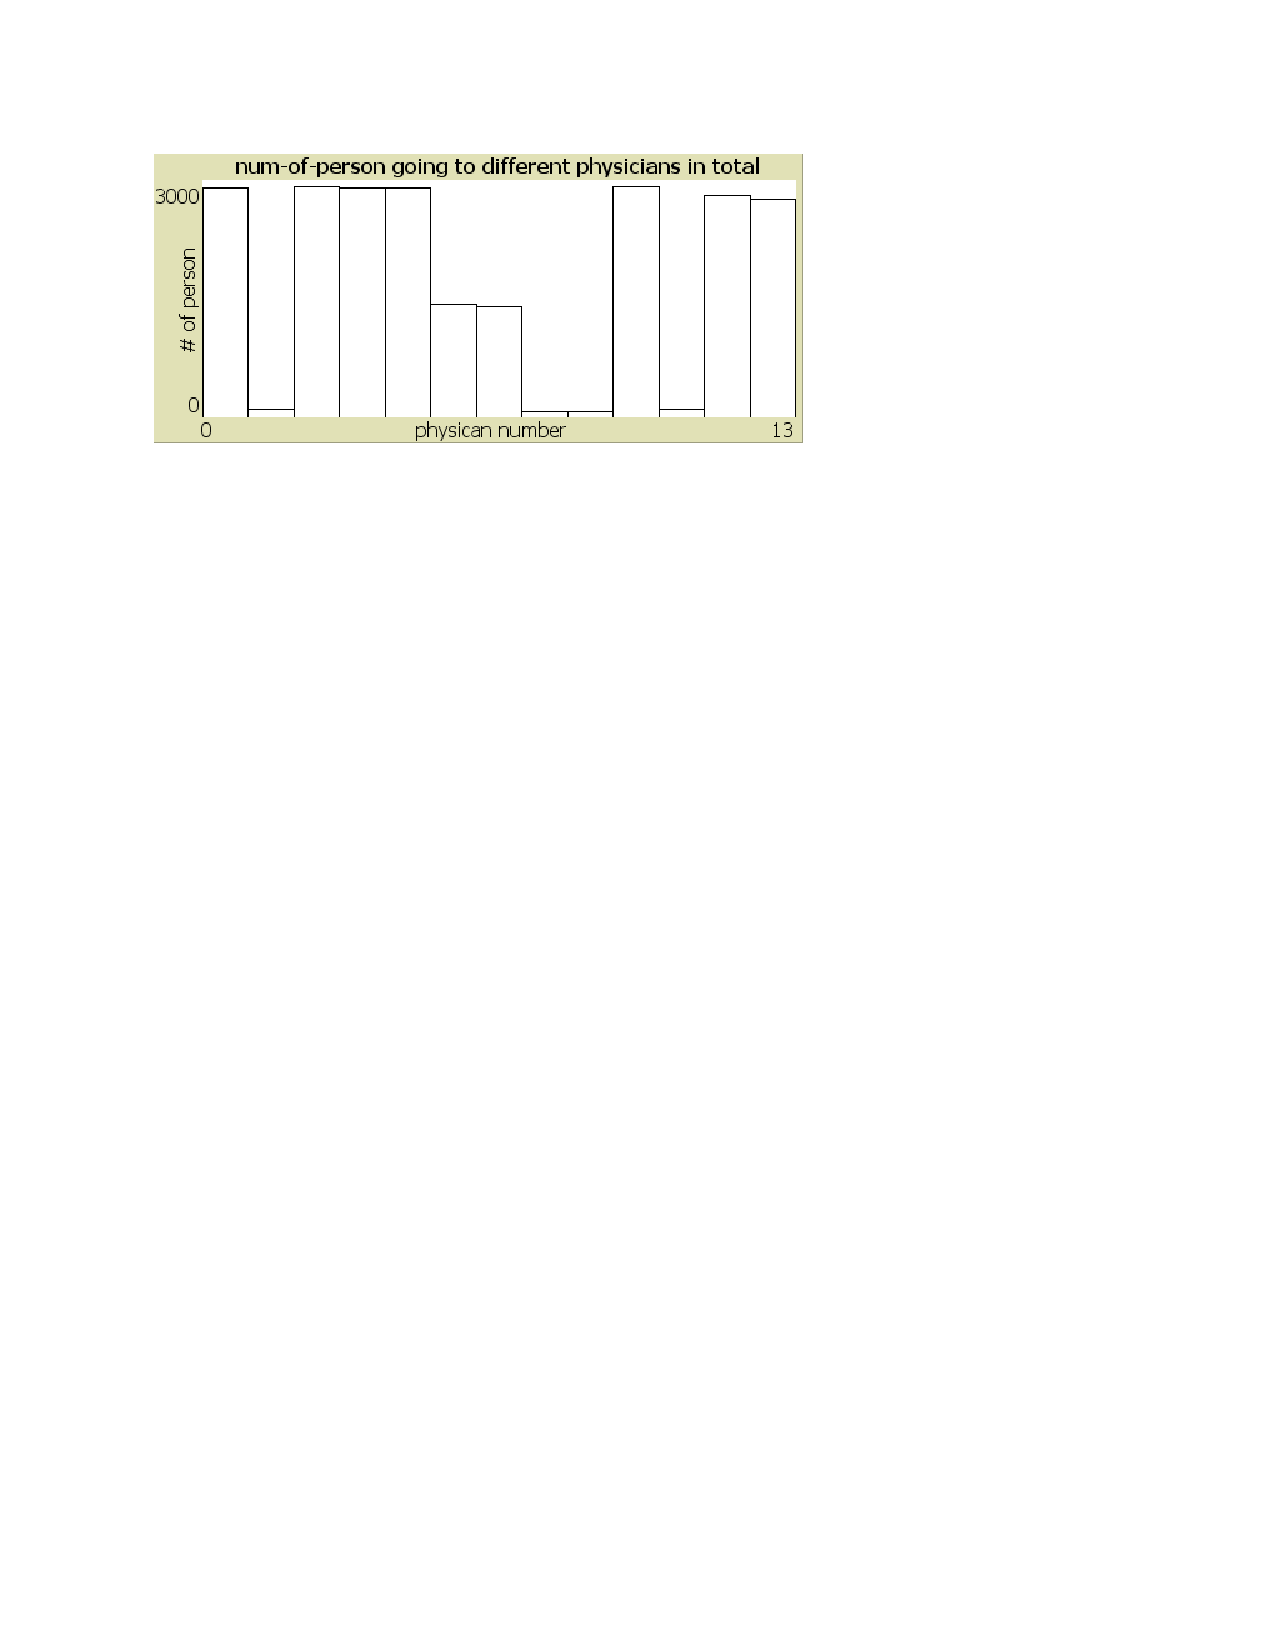
\includegraphics[scale=1]{chap3/chap3-fpatients.pdf}
\caption{Number of patients going to each physician in total}
\label{ch3:ftotalnum-of-patients}
\end{figure}

We also performed simulations with fewer physicians to check whether the claims stated above still hold. We adopted the "Choose one" and "Add and minimize" choosing-a-physician strategies and "No waiting" and "Waiting with limit" policies for conducting simulation experiments with 7 physicians. Table \ref{ch3:t7physician} shows the results in terms of average sick days. We can see that for the "No waiting" policy, the "Choose one" and "Add and minimize" choosing-a-physician strategies still perform better than the combination of "Random" strategy and "No waiting" policy. This is because a patient's Assistant Agent first chooses a physician who requires less days for curing and only then randomly chooses a physician if the patient has to wait.

Table \ref{ch3:t7physician} also shows that the combination of the "Waiting with limit" policy and all strategies for choosing a physician yields almost the same result.

\begin{table}[!t]
\centering
\caption{Average sick days with seven physicians}

\begin{tabular}{|c|c|c|}
\hline
& \multicolumn{2}{c|}{\textbf{Waiting policy}}\\ \hline
\textbf{Choosing-a-physician strategy}
& No waiting & Waiting with limit\\ \hline
Random& 28.0 & 19.2 \\ \hline
Choose one& 26.2 & 19.2 \\ \hline
Add and minimize & 18.3 & 19.2 \\ \hline
\end{tabular}
\label{ch3:t7physician}
\end{table}

In addition, we investigated the performance of a system having a lower probability that the friends of a patient in small-world network will answer a request, which are shown in Tables \ref{ch3:tdaysp0.6} and \ref{ch3:tdaysp0.4}. The "Random" strategy is shown here because it is not influenced by the probability.

\begin{table}[!t]
\centering
\caption{Average sick days with probability = 0.6}

\begin{tabular}{|c|c|c|c|}
\hline
& \multicolumn{3}{c|}{\textbf{Waiting policy}}\\ \hline
\textbf{Choosing-a-physician strategy}
& Waiting & No waiting & Waiting with limit\\ \hline
Choose one& 9.9 & 5.3 & 6.3\\ \hline
Borda voting& 7.6 & 6.3 & 6.6\\ \hline
Add and minimize & 9.8 & 5.0 & 6.4\\ \hline
\end{tabular}
\label{ch3:tdaysp0.6}
\end{table}

\begin{table}[!t]
\centering
\caption{Average sick days with probability = 0.4}

\begin{tabular}{|c|c|c|c|}
\hline
& \multicolumn{3}{c|}{\textbf{Waiting policy}}\\ \hline
\textbf{Choosing-a-physician strategy}
& Waiting & No waiting & Waiting with limit\\ \hline
Choose one&8.7 &5.4& 6.2\\ \hline
Borda voting&7.1& 6.1& 6.4\\ \hline
Add and minimize &10.4& 5.1 &6.4\\ \hline
\end{tabular}
\label{ch3:tdaysp0.4}
\end{table}

Comparing Table \ref{ch3:tdsmall} with these two tables, we discovered that the conclusions before still hold. To clarify this, we include Table \ref{ch3:ttrend}, which denotes the changing trend of the average sick days while the probability is decreasing. In the table, "+" means increasing and "" means decreasing. We can see from the table that for "Add and minimize", the average sick days increases while the probability decreases, because patients gets fewer responses from friends, leading to less informed decisions. For the "Borda voting" strategy, the average sick days decreases while the probability decreases. As mentioned before, due to the way that the "Borda voting" strategy gets the evaluation and calculates, it always gets too much information and lead to worse results than other strategies. So when the information is less with decreasing probability, we have better results of less average sick days. There's no fixed trend for a certain waiting policy with different choosing-a-physician strategies.

\begin{table}[!t]
\centering
\caption{Changing trend with decreasing probability}

\begin{tabular}{|c|c|c|c|}
\hline
& \multicolumn{3}{c|}{\textbf{Waiting policy}}\\ \hline
\textbf{Choosing-a-physician strategy}
& Waiting & No waiting & Waiting with limit\\ \hline
Choose one &- &+ &-\\ \hline
Borda voting &- &- &-\\ \hline
Add and minimize &+ &+ &+\\ \hline
\end{tabular}
\label{ch3:ttrend}
\end{table}

In the simulation, we don't guarantee that each patient rates all the physicians or the same number of physicians. The procedure of going to the physicians and learning about them follows a natural way in the real life if a patient asks his friends for recommendations. The patient's agent integrates the information and suggests a best physician according to a particular strategy and policy. As time goes on, everyone learns who are the best physicians and they tend to go to those physicians, so it is not the case that some patients have an undue influence on the ratings. 

If there is an epidemic in a certain area, conclusions become different for two waiting policies while the assumption of a uniform rate of sick people doesn't hold any more. In the particular area, large amount of patients rush into hospitals. If they adopt the "Waiting" policy, the patients will all be waiting for some of the physicians and it will take some patients a long time to get to the physicians except for the "Random" strategy. For the "Random" strategy, patients choose the physicians randomly and are distributed to physicians uniformly. Since the number of the patients increases a lot during epidemics, the average sick days and the number of leftover patients will definitely increase. However, our previous conclusions still hold which is the "Random" strategy will outperform other choosing-a-physician strategies. If the "No waiting" policy is adopted, patients tend to go to the best available physicians. However, because the number of the patients is too large, almost every physician will be occupied. Thus, all the choosing-a-physician strategies will perform the same as the "Random" strategy. For the same reason, if the "Waiting-with-limit" policy is adopted, all the choosing-a-physician will behave the same.

Another concern is that we only deal with general practitioners, but not specialists. If we include specialists in our system, the recommendation mechanism will work the same way as it is now. The only difference is that the ratings of specialists may probably be higher than the general practitioners. If a patient only cares about his goal, e.g., to get cured fast, without insisting choosing a specialist or a general practitioner, the system will work as before. If a patient has a request of choosing a specialist, the system could recommend him with the best specialist according to his strategy and policy with just adding a variable to indicate the type of a doctor. 
      

\section{Conclusion}
This chapter describes the design and rapid prototyping of a sociotechnical system for healthcare. Agent-oriented modeling was chosen for developing our simulation because it explicitly addresses the design of sociotechnical systems where the activities of humans are supported by software agents.

We investigated the prototyped sociotechnical healthcare system using agent-based simulations on the NetLogo platform. In the simulation, we investigated the influence of different strategies of finding an appropriate physician and different waiting policies in three common social network models. Our prototype revealed that if a patient adopts the "Waiting" policy, the "Random" strategy will outperform all the other strategies of choosing a physician. On the other hand, with the "No waiting" policy, all the other strategies will outperform the "Random" strategy. If the "Waiting with limit" policy is adopted, the "Choose one" and "Add and minimize" strategies will show the best performance. We found that by adopting the "Choose one" or "Add and minimize" strategy, in the "No waiting" and "Waiting with limit" case, the average number of sick days can be reduced by 0.4 - 1.8 days or 6\% - 27\%. If there is an epidemic, large amount of people get sick and rush into hospitals. If the "Waiting" strategy is adopted, which is rarely the case in the real world during epidemics because patients probably want to be cured as soon as possible, the "Random" choosing-a-physician strategy will outperform all the other strategies. For the other two policies, all the choosing-a-physician strategies perform the same.  

Our sociotechnical system differs from RateMDs and other similar websites where people can rate and find physicians in the way that people rate the physicians and patients interact. It is difficult to compare the effect of these websites and that of our system, mostly because there are no objective evaluation statistics on the websites, such as the length of time each patient takes to get cured during a period. Such websites use more flexible criteria on which different people might have different opinions, such as punctuality, medical knowledge, and time spent on a patient, while our system uses the time it takes to cure a patient as a criterion, which is more objective and meaningful. Although patients might access more ratings online, they usually do not know the people who have rated the physicians and there is a higher possibility that the ratings will not be truthful and accurate. In our system, a patient relies on friends' recommendations, which are typically more reliable.

Each agent in the sociotechnical system could be implemented on a mobile device which also has sensors to detect his principle's body temperature, glucose, and other health measures. In this way, the agent becomes an intelligent personal health assistant. It could warn the principle about abnormal health measures, provide suggestions on diet and exercise, and recommendations for physicians if his principle gets sick. Developing such multi-functional agents will greatly improve the life quality of people, especially those with potential health problems. 
